\documentclass[12pt,letterpaper]{article}

\usepackage{lipsum}
\usepackage[margin=1.5in]{geometry}
\usepackage{graphicx}
%\usepackage{crimson}
\usepackage[T1]{fontenc}
\setlength{\parindent}{0pt}
\setlength{\parskip}{6pt}
\renewcommand{\baselinestretch}{1.15}
\usepackage{titlesec}
% Level 1
\titleformat{\section}
  {\normalfont\fontsize{18}{0}\bfseries}{\thesection}{1em}{}
% Level 2
\titleformat{\subsection}
  {\normalfont\fontsize{14}{0}\bfseries}{\thesection}{1em}{}
% Level 3
\titleformat{\subsubsection}
  {\normalfont\fontsize{12}{0}\bfseries}{\thesection}{1em}{}
% Level 4
\titleformat{\paragraph}
  {\normalfont\fontsize{12}{0}\bfseries\itshape}{\theparagraph}{1em}{}
% Level 5
\titleformat{\subparagraph}
  {\normalfont\fontsize{12}{0}\itshape}{\theparagraph}{1em}{}
% Level 6
\makeatletter
\newcounter{subsubparagraph}[subparagraph]
\renewcommand\thesubsubparagraph{%
  \thesubparagraph.\@arabic\c@subsubparagraph}
\newcommand\subsubparagraph{%
  \@startsection{subsubparagraph}    % counter
    {6}                              % level
    {\parindent}                     % indent
    {12pt} % beforeskip
    {6pt}                           % afterskip
    {\normalfont\fontsize{12}{0}}}
\newcommand\l@subsubparagraph{\@dottedtocline{6}{10em}{5em}}
\newcommand{\subsubparagraphmark}[1]{}
\makeatother
\titlespacing*{\section}{0pt}{12pt}{6pt}
\titlespacing*{\subsection}{0pt}{12pt}{6pt}
\titlespacing*{\subsubsection}{0pt}{12pt}{6pt}
\titlespacing*{\paragraph}{0pt}{12pt}{6pt}
\titlespacing*{\subparagraph}{0pt}{12pt}{6pt}
\titlespacing*{\subsubparagraph}{0pt}{12pt}{6pt}

% Set caption to correct size and location
%\usepackage[tableposition=top, figureposition=bottom, font=footnotesize, labelfont=bf]{caption}



% Overwrite Title
\makeatletter
\renewcommand{\maketitle}{\bgroup
   \begin{center}
   \textbf{{\fontsize{18pt}{20}\selectfont \@title}}\\
   \vspace{10pt}
   {\fontsize{12pt}{0}\selectfont \@author} 
   \end{center}
}
\makeatother


\usepackage{float}
\usepackage{enumitem}
\usepackage{bibentry}
\nobibliography*

% Custom Quote
\newenvironment{myquote}[1]%
  {\list{}{\leftmargin=#1\rightmargin=#1}\item[]}%
  {\endlist}
  
% Create Abstract 
\renewenvironment{abstract}
{\vspace*{-.5in}\fontsize{12pt}{12}\begin{myquote}{.5in}
\noindent \par{\bfseries \abstractname.}}
{\medskip\noindent
\end{myquote}
}

%%%%%%%%%%%%%%%%%%%%%%%%%%%
%%%%%%%%%%%%%%%%%%%%%%%%%%%
\usepackage{graphicx}			% usar gráficos
\usepackage{multicol,lipsum}	%
\usepackage[utf8x]{inputenc}		% Codificacao do documento (conversão automática dos acentos)
\usepackage{indentfirst}		% Indenta o primeiro parágrafo de cada seção.
\usepackage{color}				% Controle das cores
\usepackage{graphicx}			% Inclusão de gráficos
\usepackage{graphics}           % Inclusão de gráficos
\usepackage{microtype} 			% para melhorias de justificação
\usepackage{natbib} 			% citar
\usepackage{float}				% números em ponto flutuante
\usepackage[brazil]{babel}		% língua brasileira
\usepackage{setspace}			% espaçamento entre linhas
\usepackage{subfigure}          % Permite subfiguras
\usepackage{pgfplots}           % Realizar plots
\usepackage{pdfpages}           % Inserir páginas de PDF como figura
\usepackage{comment}            % Realizar múltiplos comentários
\usepackage{listings}           % Código fonte
\usepackage{lipsum}             % Gerador de Lorem Ipsum
\usepackage{multirow}           % Multilinhas em uma tabela
\usepackage{mathtools}
\usepgfplotslibrary{polar}      % Polar axis

\graphicspath{{images/}}        % Caminho das imagens
\pagenumbering{arabic}          % Numeração das páginas
\everymath{\displaystyle}       % \frac{}{} tamanho ideal

\usepackage{amsfonts}  % Matemática 
\usepackage{amsmath}
\usepackage{amssymb}
\usepackage{caption}
\usepackage[amssymb]{SIunits}
\usepackage[pdftex]{graphicx}




% Outros pacotes
\usepackage{fullpage}
\usepackage{euscript}
\usepackage[colorlinks=true, linkcolor=blue, urlcolor=blue, pdfborder={0 0 0}]{hyperref}
%\usepackage[top=100pt,bottom=100pt,left=68pt,right=66pt]{geometry}
\usepackage{eurosym} 
\usepackage[version=3]{mhchem} 
\usepackage{enumerate}
\usepackage{epsfig}
\usepackage{setspace}
\usepackage{pdflscape}
\usepackage[]{color}
\usepackage{alltt}
\usepackage{etoolbox}
\patchcmd{\abstract}{\null\vfil}{}{}{}
\raggedbottom
\usepackage{titlesec}
\titleformat{\chapter}
{\normalfont\LARGE\bfseries}{\thechapter.}{1em}{}
\titlespacing{\chapter}{0pt}{50pt}{2\baselineskip}
\floatstyle{plaintop}
\restylefloat{table}
\usepackage[tableposition=top]{caption}
\usepackage{hyperref}
\hypersetup{hidelinks,linkcolor = black}
\usepackage{alltt}
\usepackage{etoolbox}
\usepackage{titlesec}
\raggedbottom

%----------------------------------------------


% Fancy 
\usepackage{fancyhdr}
\fancyhf{} 
\fancyfoot[C]{\rfoot{\thepage}}     % páginas numeradas right-foot
\renewcommand{\headrulewidth}{0pt}  % retira linha horizontal do fancihdr
\pagestyle{fancy}
%-------------------------------------
% Tikz
\usepackage{tikz}               
\usepackage{tikzscale}          
\usepackage[siunitx,american,cuteinductors,smartlabels]{circuitikz}
\usepackage{bodegraph}
\usetikzlibrary{intersections}
\usetikzlibrary{calc}
\usetikzlibrary{positioning}
\usetikzlibrary{babel,arrows,automata}
%-------------------------------------

%\usepackage[top=100pt,bottom=100pt,left=68pt,right=66pt]{geometry} % Geometria das folhas
%\usepackage[top=3cm, bottom=2cm, left=3cm, right=2cm]{geometry} % Geometria das folhas

%\parskip 15pt					% distância entre parágrafos fixa
%\parindent 30pt					%identação fixa

%----------------------
% Pacotes para a linha de código
%----------------------
\usepackage{xcolor}
% Definindo novas cores
\definecolor{verde}{rgb}{0,0.5,0}
% Configurando layout para mostrar codigos C++
\usepackage{listings}
\lstset{
  language=C,
  basicstyle=\ttfamily\small,
  keywordstyle=\color{blue},
  stringstyle=\color{verde},
  commentstyle=\color{red},
  extendedchars=true,
  showspaces=false,
  showstringspaces=false,
  numbers=left,
  numberstyle=\tiny,
  breaklines=true,
  backgroundcolor=\color{green!10},
  breakautoindent=true,
  captionpos=b,
  xleftmargin=0pt,
}
%----------------------
% Aumentar tamanho do título resumo
\makeatletter
\renewenvironment{abstract}{%
    \if@twocolumn
      \section*{\abstractname}%
    \else %% <- here I've removed \small
      \begin{center}%
        {\bfseries \Large\abstractname\vspace{\z@}}%  %% <- here I've added \Large
      \end{center}%
      \quotation
    \fi}
    {\if@twocolumn\else\endquotation\fi}
\makeatother
%----------------------
%%%%%%%%%%%%%%%%%%%%%%%%%%%
%%%%%%%%%%%%%%%%%%%%%%%%%%%

\setcitestyle{square}


%\usepackage{fontspec}
%\setmainfont{[calibril.ttf]}

\begin{document}
\section{Introdução}

Os sistemas reais nem sempre possuem o comportamento de saída como o desejado, seja pelas não idealidades dos componentes ou pela própria dinâmica do sistema. Considerando a impossibilidade de alterar essas particularidades, seja por os componentes não serem acessíveis à modificação ou se o acesso seja invasivo ao sistema, surge a necessidade de projetar controladores.

O controladores procuram avaliar as saídas atuais do sistema e, com base em certos parâmetros, atuar na entrada do sistema para que a saída se comporte como desejada. Não necessitando que altere a dinâmica do sistema original. 

Dessa forma, o presente trabalho tem o objetivo de projetar controladores por realimentação negativa e por realimentação de estados para a planta modelada pela função de transferência da equação \ref{planta:eq}. Os métodos de projeto de controladores PID por realimentação negativa (\textit{negative feedback}) compreendem: método pelo lugar das raízes, método polinomial e método frequencial. Já para o controlador por realimentação de estados (\textit{state feedback}) foi utilizado o método utilizando a fórmula de Ackermann

\begin{equation}\label{planta:eq}
    G_p(s) = \frac{2}{s(s+0,5)}
\end{equation}

Por meio do Scilab simula-se inicialmente o sistema em malha aberta e fechada sem o uso de controladores, de forma a avaliar se há a necessidade de projetar um controaldor.

Para simular o sistema em malha aberta, montou-se o diagrama mostrado na figura ~\ref{xcos:ma:a} e se obteve a saída conforme ilustra a figura ~\ref{xcos:ma:b}. Assim, percebe-se uma instabilidade no sistema, promovida pela presença do integrador na planta.

\begin{figure}[H]
\begin{center}
    \subfigure[Diagrama de blocos]{             
        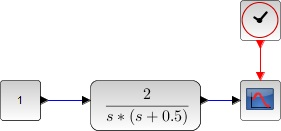
\includegraphics[width=5.5cm]{images/metodo_frequencial/xcosOL.jpg}  
        \label{xcos:ma:a}
    }
    \subfigure[Simulação temporal]{                                              
        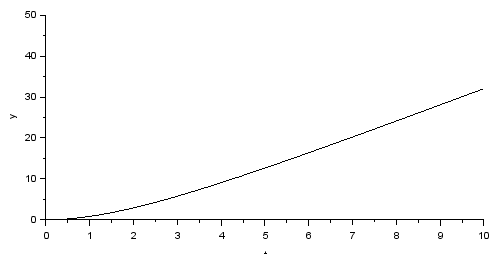
\includegraphics[width=9.5cm]{images/metodo_frequencial/timeOL.png}
        \label{xcos:ma:b}
    }                
\end{center}
\caption{Simulação com a planta em malha aberta no XCOS.}
\label{xcos:ma} 
\end{figure}

Colocando a planta em malha fechada, conforme mostra a figura ~\ref{xcos:mf:a}, obteve-se o desempenho expresso na figura ~\ref{xcos:mf:b}, apresentando um percentual de \textit{overshoot} de cerca de $57\%$ e tempo de estabilização de, aproximadamente, $14$ segundos. Assim, demonstrando a necessidade de um controle

\begin{figure}[H]
\begin{center}
    \subfigure[Diagrama de blocos]{             
        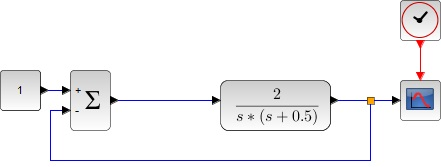
\includegraphics[width=6cm]{images/metodo_frequencial/xcosCL.jpg}  
        \label{xcos:mf:a}
    }
    \subfigure[Simulação temporal]{                                              
        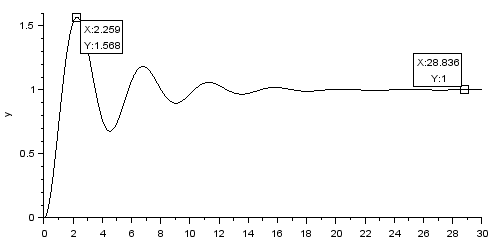
\includegraphics[width=9.5cm]{images/metodo_frequencial/timeCL.png}
        \label{xcos:mf:b}
    }                
\end{center}
\caption{Simulação com a planta em malha fechada no XCOS.}
\label{xcos:mf} 
\end{figure}
%\pagebreak
\section{Metodologia}

\lipsum[1]


\pagebreak

\section{Resultados e discussão}

Para encontrar todos os resultados necessários para comprovar a teoria, a prática foi dividida em algumas etapas, sendo elas:


\begin{itemize}

    \item Inicialmente foram montados os circuitos da figura \ref{ckt:1} e \ref{ckt:2};
    
    \item Para cada um dos circuitos foi utilizada uma senoide de 5V de pico (10V de pico-a-pico) e frequência variável na entrada, de forma que: $V_i(t) = 5sen(2\pi f t)$, para traçar a função de transferência de módulo e de fase para cada um dos circuitos;
    
    \item Com a mesma senoide do item anterior a frequência foi variada para encontrar a exata frequência de corte de cada filtro.
\end{itemize}

Para medir a frequência de corte de cada circuito os critérios de ganho e de fase foram utilizados, de forma que a frequência de corte ocorre na curva de Bode de ganho quando esta possui uma queda de 3dB. O critério de fase diverge para o filtro de 1ª ordem e o filtro de 2ª ordem, sendo que neste a frequência de corte ocorre em -90° e naquele ocorre em -45º na curva de Bode de fase.

Considerando o filtro passa-baixa de 1ª ordem, a frequência da tensão de entrada foi variada de 1Hz a 20kHz, permitindo obter os dados da tabela \ref{table:1}. Com esses dados foi possível montar as curvas de Bode da figura \ref{graph:1}. 

\begin{figure}[H]
\begin{center}
\begin{tikzpicture} [scale=0.8]
\begin{semilogxaxis}[
    title={},
    xlabel={$\omega$ (rad/s)},
    ylabel={$|T_{first-order}|$ (dB)},
    xmin=1, xmax=100000,
    ymin=-25, ymax=5,
    xtick={1,10,100,1000,10000,100000,1000000},
    ytick={0, -3, -10, -20},
    legend pos=north west,
    ymajorgrids=true,
    grid style=dashed,
]
\addplot[
    color=blue,
    mark=square,
    ]
    coordinates {
    (6.28,0)
    (31.42,0)
    (62.83,0)
    (94.25,0)
    (188.5,0)
    (314.16,0)
    (471.24,0)
    (628.32,0)
    (1256.64,-0.156)
    (1570.80,-0.253)
    (1884.96,-0.351)
    (2513.27,-0.596)
    (3141.59,-0.839)
    (4712.39,-1.694)
    (6283.19,-2.615)
    (6945.43,-3.012)
    (9424.78,-4.510)
    (10995.57,-5.465)
    (12566.37,-6.196)
    (31415.93,-13.120)
    (47123.89,-16.393)
    (62831.85,-18.808)
    (75398.22,-20.419)
    (94247.78,-22.099)
    (113097.34,-23.703)
    (125663.71,-24.324)
    };
\end{semilogxaxis}
\end{tikzpicture}
\hspace{1cm}
\begin{tikzpicture} [scale=0.8]
\begin{semilogxaxis}[
    title={},
    xlabel={$\omega$ (rad/s)},
    ylabel={$\angle T_{first-order}$ (°)},
    xmin=10, xmax=100000,
    ymin=-95, ymax=5,
    xtick={10,100,1000,10000,100000,1000000},
    ytick={0, -45, -90},
    legend pos=north west,
    ymajorgrids=true,
    grid style=dashed,
]
\addplot[
    color=blue,
    mark=square,
    ]
    coordinates {
    (6.28,0)
    (31.42,0)
    (62.83,0)
    (94.25,0)
    (188.5,-1)
    (314.16,-2)
    (471.24,-4)
    (628.32,-5)
    (1256.64,-10)
    (1570.80,-12)
    (1884.96,-17)
    (2513.27,-23)
    (3141.59,-25)
    (4712.39,-34)
    (6283.19,-43)
    (6945.43,-45)
    (9424.78,-53)
    (10995.57,-59)
    (12566.37,-60)
    (31415.93,-79)
    (47123.89,-83)
    (62831.85,-84)
    (75398.22,-86)
    (94247.78,-87)
    (113097.34,-88)
    (125663.71,-89)
    };
\end{semilogxaxis}
\end{tikzpicture}
\end{center}
\caption{Curvas de bode com os resultados práticos da função de transferência do filtro passa-baixas de 1ª ordem.}
\label{graph:1} 
\end{figure}

No filtro passa-baixa de 1ª ordem esperava-se que para uma tensão de entrada de 10V de pico-a-pico, a saída fosse de 7.07 V de pico-a-pico e que a defasagem entre a forma de onda de tensão da entrada e da saída fosse de -45°. Isso foi perfeitamente obtido na prática, da forma como foi encontrada na tabela e cujas formas de onda podem ser observadas na figura \ref{fo1}.

\begin{figure}[H] 
\centering
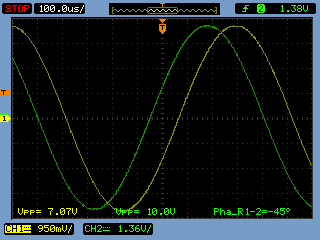
\includegraphics[width=7cm]{images/f0_1.png}
\caption{Formas de onda obtidas no osciloscópio para o filtro passa-baixa de 1ª ordem na frequência de corte, sendo a saída no CH1 e a entrada no CH2.}
\label{fo1} 
\end{figure}

A frequência de corte obtida na prática foi de 1105.4Hz, uma vez que a esperada era de 1061Hz, o erro relacionado à frequência é de 4.01\%.

A partir dos dados da tabela \ref{table:1}, se escolher o ganho para a frequência de 2kHz (-6.196 dB) e o ganho uma década depois, ou seja, em 20kHz (-24.324 dB), observa-se um queda de 18.128 dB, um valor bem próximo do esperado pela curva teórica, que é uma atenuação de 20 dB por década, com um erro de 9.36\%. Ao conferir as curvas de Bode da figura \ref{graph:1}, observa-se uma boa concordância com as curvas da figura \ref{fig:3} obtidas no MATLAB.

Para o  filtro passa-baixa de 2ª ordem, a frequência da tensão de entrada também foi variada de 1Hz a 20kHz, permitindo obter os dados da tabela \ref{table:2}. Com esses dados foi possível montar as curvas de Bode da figura \ref{graph:2}. 

\begin{figure}[H]
\begin{center}
\begin{tikzpicture} [scale=0.8]
\begin{semilogxaxis}[
    title={},
    xlabel={$\omega$ (rad/s)},
    ylabel={$|T_{second-order}|$ (dB)},
    xmin=1, xmax=100000,
    ymin=-55, ymax=5,
    xtick={1,10,100,1000,10000,100000,1000000},
    ytick={0, -3, -25, -50},
    legend pos=north west,
    ymajorgrids=true,
    grid style=dashed,
]
\addplot[
    color=blue,
    mark=square,
    ]
    coordinates {
    (6.28,0.086)
    (31.42,0.086)
    (62.83,0.086)
    (94.25,0.086)
    (188.5,0.086)
    (314.16,0.086)
    (471.24,0.086)
    (628.32,0.086)
    (1256.64,0.086)
    (1570.80,0.086)
    (1884.96,0)
    (2513.27,0)
    (3141.59,-0.244)
    (4712.39,-1.031)
    (6283.19,-2.796)
    (6477.96,-3.012)
    (9424.78,-7.447)
    (10995.57,-9.710)
    (12566.37,-11.843)
    (31415.93,-27.171)
    (47123.89,-34.895)
    (62831.85,-39.830)
    (75398.22,-42.844)
    (94247.78,-46.462)
    (113097.34,-52.197)
    (125663.71,-54.420)
    };
\end{semilogxaxis}
\end{tikzpicture}
\hspace{1cm}
\begin{tikzpicture} [scale=0.8]
\begin{semilogxaxis}[
    title={},
    xlabel={$\omega$ (rad/s)},
    ylabel={$\angle T_{first-order}$ (°)},
    xmin=10, xmax=100000,
    ymin=-185, ymax=5,
    xtick={10,100,1000,10000,100000,1000000},
    ytick={0, -90, -180},
    legend pos=north west,
    ymajorgrids=true,
    grid style=dashed,
]
\addplot[
    color=blue,
    mark=square,
    ]
    coordinates {
    (6.28,0)
    (31.42,0)
    (62.83,-1)
    (94.25,-2)
    (188.5,-2)
    (314.16,-4)
    (471.24,-7)
    (628.32,-8)
    (1256.64,-17)
    (1570.80,-20)
    (1884.96,-24)
    (2513.27,-33)
    (3141.59,-45)
    (4712.39,-69)
    (6283.19,-89)
    (6477.96,-91)
    (9424.78,-120)
    (10995.57,-130)
    (12566.37,-137)
    (31415.93,-165)
    (47123.89,-170)
    (62831.85,-176)
    (75398.22,-178)
    (94247.78,-179)
    (113097.34,-180)
    (125663.71,-180)
    };
\end{semilogxaxis}
\end{tikzpicture}
\end{center}
\caption{Curvas de bode com os resultados práticos da função de transferência do filtro passa-baixas de 2ª ordem}
\label{graph:2} 
\end{figure}

No filtro passa-baixa de 2ª ordem, esperava-se que para uma tensão de entrada de 10V de pico-a-pico, a saída fosse de 7.07 V de pico-a-pico e que a defasagem entre a forma de onda de tensão da entrada e da saída fosse de -90°. Isso foi quase que perfeitamente obtido na prática, da forma como foi encontrada na tabela e cujas formas de onda podem ser observadas na figura \ref{fo2}, com uma defasagem de -91° ao invés de 90°, com um erro de 1.09\%.

\begin{figure}[H] 
\centering
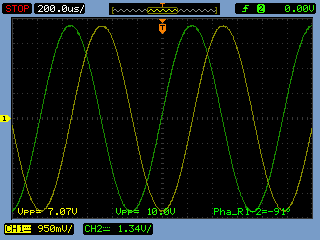
\includegraphics[width=7cm]{images/f0_2.png}
\caption{Formas de onda obtidas no osciloscópio para o filtro passa-baixa de 2ª ordem na frequência de corte, sendo a saída no CH1 e a entrada no CH2.}
\label{fo2} 
\end{figure}

A frequência de corte obtida na prática foi de 1031Hz, uma vez que a esperada era de 967.51Hz, o erro relacionado à frequência é de 6.15\%.

A partir dos dados da tabela \ref{table:1}, se escolher o ganho para a frequência de 2kHz (-11.843 dB) e o ganho uma década depois, ou seja, em 20kHz (-54.420 dB), observa-se um queda de 42.577 dB, um valor bem próximo do esperado pela curva teórica, que é uma atenuação de 40 dB por década, com um erro de 6.05\%. Ao conferir as curvas de Bode da figura \ref{graph:2}, observa-se uma boa concordância com as curvas da figura \ref{fig:4} obtidas no MATLAB.

Uma medida importante do filtro de 2ª ordem é o seu fator de qualidade (Q). Reconhecendo a forma geral da função de transferência de um filtro de segunda ordem na equação \ref{q1} e os seus polos na equação \ref{q2}, observa-se que a um valor alto de Q permite que a distância dos polos até o eixo $j\omega$ diminua, tornando assim o filtro mais seletivo.

\begin{equation} \label{q1}
    T(s) = \frac{a_2s^2+a_1s+a_0}{s^2+(\omega/Q)s+\omega^2}
\end{equation}

\begin{equation} \label{q2}
    p_1, p_2 = -\frac{\omega}{2Q}\pm j\omega\sqrt{1-(1/4Q)^2}
\end{equation}

Para o caso do filtro de 2ª ordem implementado na prática, o valor de Q é 0.709, que é um valor próximo de 0.707, cuja resposta obtida para esse fator de qualidade é chamada Butterworth, ou a resposta mais achatada e que foi constatada na prática. Na figura \ref{Q} observa-se que ao diminuir o fator Q da função de transferência do filtro passa-baixa de segunda ordem o filtro se torna menos seletivo e, de acordo com que Q aumenta, a seletividade aumenta, porém a resposta apresenta picos de ressonância na frequência de corte. 

\begin{figure}[H] 
\centering
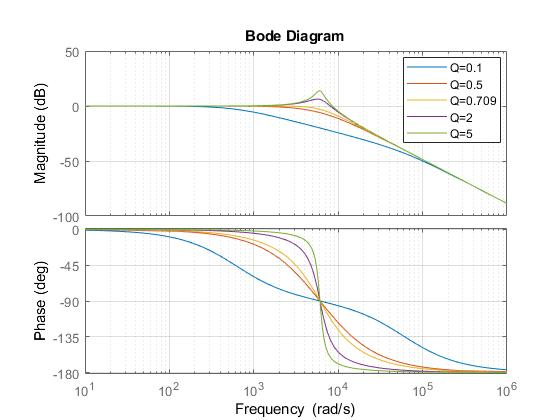
\includegraphics[width=14cm]{images/BodeQ.jpg}
\caption{Ensaios para valores variáveis de Q na função de transferência do filtro passa-baixas de 2ª ordem.}
\label{Q} 
\end{figure}

Por fim a figura \ref{graph:3} mostra a comparação direta das curvas de Bode do filtro passa-baixas de 1ª e 2ª ordem, mostrando que de fato o filtro de 2ª ordem possui uma maior seletividade representada na capacidade de atenuar frequências acima da de corte com um fator 40dB por década, ao passo que o filtro de 1ª ordem só atenua 20dB por década. Porém esta conclusão não tira o mérito do filtro de 1ª ordem, pois ele ainda se apresenta uma alternativa um pouco mais barata ao filtro de 2ª ordem.

\begin{figure}[H]
\begin{center}
\begin{tikzpicture} [scale=0.8]
\begin{semilogxaxis}[
    title={},
    xlabel={$\omega$ (rad/s)},
    ylabel={$|T|$ (dB)},
    xmin=1, xmax=100000,
    ymin=-55, ymax=5,
    xtick={1,10,100,1000,10000,100000,1000000},
    ytick={0, -3, -10, -25, -40, -50},
    legend pos=north west,
    ymajorgrids=true,
    grid style=dashed,
    legend style={at={(0.03,0.05)},anchor=south west},
]
\addplot[
    color=cyan,
    mark=square,
    ]
    coordinates {
    (6.28,0)
    (31.42,0)
    (62.83,0)
    (94.25,0)
    (188.5,0)
    (314.16,0)
    (471.24,0)
    (628.32,0)
    (1256.64,-0.156)
    (1570.80,-0.253)
    (1884.96,-0.351)
    (2513.27,-0.596)
    (3141.59,-0.839)
    (4712.39,-1.694)
    (6283.19,-2.615)
    (6945.43,-3.012)
    (9424.78,-4.510)
    (10995.57,-5.465)
    (12566.37,-6.196)
    (31415.93,-13.120)
    (47123.89,-16.393)
    (62831.85,-18.808)
    (75398.22,-20.419)
    (94247.78,-22.099)
    (113097.34,-23.703)
    (125663.71,-24.324)
    }; \addlegendentry{First-order}
\addplot[
    color=blue,
    mark=square,
    ]
    coordinates {
    (6.28,0.086)
    (31.42,0.086)
    (62.83,0.086)
    (94.25,0.086)
    (188.5,0.086)
    (314.16,0.086)
    (471.24,0.086)
    (628.32,0.086)
    (1256.64,0.086)
    (1570.80,0.086)
    (1884.96,0)
    (2513.27,0)
    (3141.59,-0.244)
    (4712.39,-1.031)
    (6283.19,-2.796)
    (6477.96,-3.012)
    (9424.78,-7.447)
    (10995.57,-9.710)
    (12566.37,-11.843)
    (31415.93,-27.171)
    (47123.89,-34.895)
    (62831.85,-39.830)
    (75398.22,-42.844)
    (94247.78,-46.462)
    (113097.34,-52.197)
    (125663.71,-54.420)
    }; \addlegendentry{Second-order}
\end{semilogxaxis}
\end{tikzpicture}
\hspace{1cm}
\begin{tikzpicture} [scale=0.8]
\begin{semilogxaxis}[
    title={},
    xlabel={$\omega$ (rad/s)},
    ylabel={$\angle T$ (°)},
    xmin=10, xmax=100000,
    ymin=-185, ymax=5,
    xtick={10,100,1000,10000,100000,1000000},
    ytick={0, -45, -90, -135, -180},
    legend pos=north west,
    ymajorgrids=true,
    grid style=dashed,
    legend style={at={(0.03,0.05)},anchor=south west},
]
\addplot[
    color=cyan,
    mark=square,
    ]
    coordinates {
    (6.28,0)
    (31.42,0)
    (62.83,0)
    (94.25,0)
    (188.5,-1)
    (314.16,-2)
    (471.24,-4)
    (628.32,-5)
    (1256.64,-10)
    (1570.80,-12)
    (1884.96,-17)
    (2513.27,-23)
    (3141.59,-25)
    (4712.39,-34)
    (6283.19,-43)
    (6945.43,-45)
    (9424.78,-53)
    (10995.57,-59)
    (12566.37,-60)
    (31415.93,-79)
    (47123.89,-83)
    (62831.85,-84)
    (75398.22,-86)
    (94247.78,-87)
    (113097.34,-88)
    (125663.71,-89)
    }; \addlegendentry{First-order}
\addplot[
    color=blue,
    mark=square,
    ]
    coordinates {
    (6.28,0)
    (31.42,0)
    (62.83,-1)
    (94.25,-2)
    (188.5,-2)
    (314.16,-4)
    (471.24,-7)
    (628.32,-8)
    (1256.64,-17)
    (1570.80,-20)
    (1884.96,-24)
    (2513.27,-33)
    (3141.59,-45)
    (4712.39,-69)
    (6283.19,-89)
    (6477.96,-91)
    (9424.78,-120)
    (10995.57,-130)
    (12566.37,-137)
    (31415.93,-165)
    (47123.89,-170)
    (62831.85,-176)
    (75398.22,-178)
    (94247.78,-179)
    (113097.34,-180)
    (125663.71,-180)
    }; \addlegendentry{Second-order}
\end{semilogxaxis}
\end{tikzpicture}
\end{center}
\caption{Comparação entre as funções de transferência de cada filtro.}
\label{graph:3} 
\end{figure}


%\newpage
\section{Conclusões}

O controle digital por computador se mostrou uma boa alternativa ao controle analógico tradicional, pois ele permite a facilidade de reprojeto e um ambiente com condições externas controladas, evitando ter que se preocupar com fatores limitantes do ambiente ou de tolerância de componentes. Porém, como a representação digital é apenas uma aproximação da representação analógica, a velocidade no processamento dos dados será um barreira limitante, pois ela dita a precisão do modelo. Entretanto, ao obedecer o teorema da amostragem e conhecimento prévio do hardware no qual o controlador será implementado, as barreiras limitantes diminuem, permitindo a expansão das técnicas de controle tradicionais para novos horizontes de aplicações.
\pagebreak
\newpage
%\begin{thebibliography}{99}
\bibitem{b1} de Lauro Castrucci, Plínio Benedicto, e Anselmo Bittar. Controle automático. Grupo Gen-LTC, 2000.
\bibitem{b2} Kuo, Benjamin C., e Farid Golnaraghi. Automatic control systems. Vol. 9. Englewood Cliffs, NJ: Prentice-Hall, 1995.
\bibitem{b3} Introduction to Control Systems in Scilab. Disponível em: \url{http://www.openeering.com/}.
\bibitem{b4} Ogata, Katsuhiko. Modern control engineering. Upper Saddle River, NJ: Prentice Hall, 2009.
\bibitem{b5} Sedra, Adel S., et al. Microelectronic circuits. Oxford University Press, 2016.
\end{thebibliography}

\pagebreak
\end{document}
